\section{习题 2.5：旋转面、柱面与锥面（17 题）}\label{sec:25}
\tip{\textbf{三个统一构造思想：}（1）\emph{旋转面}保持到旋转轴的距离，以及在轴上的投影不变；（2）\emph{柱面}沿固定非零向量 $u$ 平移而成，可将点 $X$ 沿 $u$ 回退到准线；（3）\emph{锥面}从顶点 $V$ 向准线上点作直线，可令 $X=V+t(P-V)$ 消去参数。}
\begin{center}
\begin{tikzpicture}[scale=.88,>=Stealth]
\draw[thick,->] (1,-.2)--(1,4.2) node[above]{$z$};
\draw[blue,thick] plot[smooth] coordinates {(1.6,.3)(2.2,1)(2.5,2)(2.2,3)(1.6,3.6)};
\draw[blue,thick,dashed] plot[smooth] coordinates {(.4,.3)(-.2,1)(-.5,2)(-.2,3)(.4,3.6)};
\foreach \y/\rx in {.4/.45,1/.95,2/1.4,3/.95,3.5/.55}{\draw[teal!65] (1,\y) ellipse (\rx cm and .19cm);}
\node at (4.0,3) {母线绕轴旋转};
\node at (4.1,2.45) {产生旋转面};
\draw[->,red] (3.4,2.1)--(2.4,2.0);
\end{tikzpicture}
\end{center}

\begin{center}
\begin{minipage}{.47\linewidth}\centering
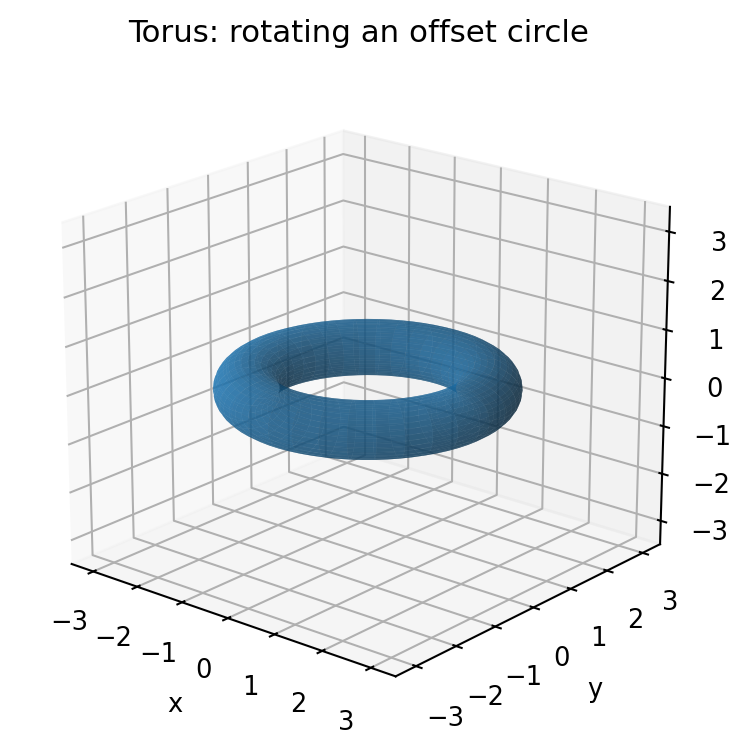
\includegraphics[width=\linewidth]{figures/torus.png}
{\small\color{navy}环面：圆绕不穿过圆面的轴旋转}
\end{minipage}\hfill
\begin{minipage}{.47\linewidth}\centering
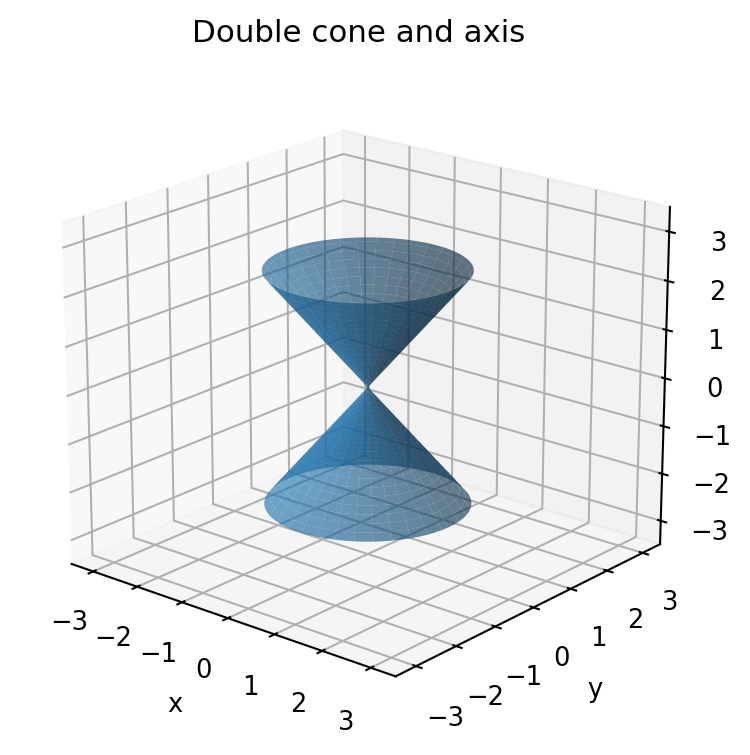
\includegraphics[width=\linewidth]{figures/double-cone.png}
{\small\color{navy}双圆锥：直线母线经过同一顶点}
\end{minipage}
\end{center}
\Q{1}{七种曲线绕不同直线旋转}
\idea{绕 $z$ 轴时保留 $z$、以 $\rho^2=x^2+y^2$ 替代原曲线到轴的距离。绕其他轴时，先把坐标平移旋转到以目标轴为新 $z$ 轴的坐标，再还原。}
\begin{enumerate}[label=(\arabic*)]
\item 直线 $\frac x1=\frac{y+2}{-3}=\frac{z+7}{-2}$ 绕 $z$ 轴：令参数 $t=x$，有 $y=-2-3t,z=-7-2t$，由 $t=-(z+7)/2$ 得
\[x^2+y^2=\frac{(z+7)^2+(3z+17)^2}{4}.\]
\ans{$2x^2+2y^2-5z^2-58z-169=0$。}
\item 直线 $x=1,z=0$ 绕题给直线 $x+z=0,\ 2x-2y+z=0$ 旋转：求旋转轴方向 $u$ 及轴上一点 $O$，令旋转点 $X$ 与母线点 $P$ 同轴向投影且同轴距；消去母线参数得到
\ans{$3x^2+3z^2+4xy-8xz-4yz-8x-4y+8z+5=0$。}
\item 圆 $(x-3)^2+y^2=4,z=0$ 绕 $x$ 轴：距离轴的圆截面转为 $y^2+z^2$，故
\ans{$(x-3)^2+y^2+z^2=4$（球面）。}
\item 同一个圆绕 $y$ 轴：圆心距旋转轴 $3$，圆半径 $2$，得到环面。令 $\rho=\sqrt{x^2+z^2}$，其轴向截面为
\[(\rho-3)^2+y^2=4.
\]
移项后平方，得到
\[\boxed{(x^2+y^2+z^2+5)^2-36(x^2+z^2)=0}.\]
\ans{这是原书展开为四次多项式的简洁等价写法。}
\item 抛物线 $y=x^2+4,z=0$ 绕 $y$ 轴，\ans{$y=x^2+z^2+4$（抛物面）。}
\item 同一抛物线绕 $x$ 轴，\ans{$y^2+z^2=(x^2+4)^2$。}
\item 曲线 $y=x^3,z=0$ 绕 $y$ 轴：$|y|=\rho^3$，平方后得\ans{$y^2=(x^2+z^2)^3$。}
\end{enumerate}
\tip{第 (4) 问的环面尤其适合观察：大半径 $3$ 是圆心到转轴的距离，小半径 $2$ 是原圆半径。先写 $\rho$ 的截面关系，比直接展开高次多项式好理解。}

\Q{2}{曲线绕 $y$ 轴旋转后是否为单位圆柱面？}
原曲线为 $x^2+y^2=1,z=x^2$。绕 $y$ 轴时，$y$ 保持不变，而到 $y$ 轴的距离满足
\[\rho^2=x^2+z^2=x^2+x^4.\]
由 $x^2=1-y^2$ 可得
\[\rho^2=(1-y^2)+(1-y^2)^2,\qquad |y|\le1.\]
它并非恒为 $1$，所以不可能是 $x^2+z^2=1$。
\ans{不是。只把原式中的 $x^2+y^2$ 看作旋转不变量是错误的，因为绕的是 $y$ 轴。}

\Q{3}{绕 $y$ 轴旋转后得到圆柱面上的哪一部分？}
原曲线为 $x^2+y^2-z^2=0,\ x^2+z^2=1$。绕 $y$ 轴后，柱面不变量是 $x^2+z^2=1$。由两式相减得到 $y^2=1-2x^2$，因此必有 $|y|\le1$。
反过来，每一个 $|y|\le1$ 的高度都对应原曲线的某个点，而它绕 $y$ 轴生成完整的圆。
\ans{$x^2+z^2=1,\ |y|\le1$，圆柱面的有限带状部分。}

\Q{4}{两种直线绕 $z$ 轴旋转}
\begin{enumerate}[label=(\arabic*)]
\item $z=3x+2,\ z=2y-1$：原直线上任一点有 $x=(z-2)/3$、$y=(z+1)/2$，故
\[x^2+y^2=\frac{(z-2)^2}{9}+\frac{(z+1)^2}{4}.\]
\ans{$36x^2+36y^2-13z^2-2z-25=0$。}
\item $z=ax+b,\ z=cy+d$（$ac\ne0$）：同理，
\[\boxed{x^2+y^2=\frac{(z-b)^2}{a^2}+\frac{(z-d)^2}{c^2}}.\]
展开得到原书答案中关于 $a,b,c,d$ 的一般二次式。
\end{enumerate}

\Q{5}{到两定点距离的和 / 比为常数}
\begin{enumerate}[label=(\arabic*)]
\item 到 $A(-3,0,0),B(3,0,0)$ 的距离和为 $10$。焦距 $2c=6$，长半轴 $a=5$，由 $b^2=a^2-c^2=25-9=16$，绕焦轴 $x$ 旋转得到\textbf{旋转椭球面}：
\[\boxed{\frac{x^2}{25}+\frac{y^2+z^2}{16}=1}.\]
\warning{书后答案页（原书纸质第 300 页）印成 $x^2/5+y^2/4+z^2/4=1$，与“两焦点距离和为 $10$”不符。举例 $(5,0,0)$ 满足距离和为 $10$，却不满足印出的式子。本讲义独立计算所得分母应为 $25,16,16$。}
\item 到 $A(1,0,0),B(4,0,0)$ 距离比为 $1:2$：
\[4[(x-1)^2+y^2+z^2]=(x-4)^2+y^2+z^2.\]
整理得\ans{$x^2+y^2+z^2=4$，是球心在原点、半径为 $2$ 的球面。}
\end{enumerate}

\Q{6}{点到点与点到平面距离的比例轨迹}
取 $\pi:z=0$、$M=(0,0,4)$。
(1) 等距条件：
\[\sqrt{x^2+y^2+(z-4)^2}=|z| \iff x^2+y^2-8z+16=0.\]
(2) 距离比 $3:1$：
\[\sqrt{x^2+y^2+(z-4)^2}=3|z|\iff x^2+y^2-8z^2-8z+16=0.\]
\ans{(1) 旋转抛物面；(2) 双叶双曲面的一个参数形式，原书给出的二次式一致。}

\Q{7}{四种圆柱面的方程}
\idea{圆柱面上的点 $X$ 到固定轴线 $l:P_0+tu$ 的距离恒为半径 $r$：
\[\boxed{|(X-P_0)\times u|^2=r^2|u|^2}.\]
此式避免先求直角化坐标。}
\begin{enumerate}[label=(\arabic*)]
\item 以 $\frac{x}{1}=\frac{y}{-1}=\frac{z+1}{-2}$ 为轴，经过与它平行的直线 $\frac{x-1}{1}=\frac{y+2}{-1}=\frac{z+4}{-2}$：轴距为圆柱半径。代入叉乘公式并化简得到
\[5x^2+5y^2+2z^2+2xy+4xz-4yz+4x-4y+4z-1=0.\]
\item 轴线经过 $(1,0,2)$ 且平行 $u=(1,2,3)$，半径 $3$。直接写
\[|(x-1,y,z-2)\times(1,2,3)|^2=9(1+4+9).\]
展开等价于书后给出的 $13x^2+10y^2+5z^2-4xy-6xz-12yz-14x+28y-14z-105=0$。
\item 轴线为 $\frac{x-1}{1}=\frac{y-2}{-1}=\frac{z+2}{2}$，圆柱面过 $(1,-1,0)$。先用点到轴线距离确定半径，再写叉乘方程即可。\ans{独立核算得到 $5x^2+5y^2+2z^2+2xy-4xz+4yz-22x-14y+4z=0$。}
\warning{原书答案页对应式子多印一个常数 $-5$。但题设给定的曲面上点 $(1,-1,0)$ 代入原书多项式为 $-5\ne0$；独立按点到轴线距离公式展开则无常数项。本稿改用可验证的结果。}
\item 母线平行 $u=(1,1,1)$，圆柱面经过 $(0,0,0),(-1,0,1),(1,-1,0)$。先把这三点投影到垂直 $u$ 的截面，三投影确定截面圆；回到空间得到
\ans{$x^2+y^2+z^2-xy-xz-yz+3y-3z=0$。}
\end{enumerate}

\Q{8}{给定球面的一对平行切平面}
球面球心 $C=(0,1,-1)$，半径 $2$。平行 $u=(1,1,1)$ 的切平面即法向量为 $u$ 的平面，故设
\[x+y+z=D.\]
切平面到球心距离应为 $2$：$|D-(0+1-1)|/\sqrt3=2$。因此
\ans{$x+y+z=\pm2\sqrt3$，两张切平面。}

\Q{9}{以给定椭圆为准线的圆柱面有几张？}
椭圆准线 $x^2+4y^2=4,z=0$。任取一个不平行于 $z=0$ 的方向向量 $u$，将椭圆每一点沿 $u$ 平移即可得到一张柱面。因此满足“经过这条曲线”的柱面\textbf{不唯一，而是无穷多张}。
\ans{无穷多个；题中若另外给出母线方向，则才能确定唯一圆柱面。}

\Q{10}{四种圆锥面的方程}
\idea{过顶点 $V$、轴方向 $u$、半顶角 $\alpha$ 的旋转圆锥满足
\[\boxed{[(X-V)\cdot u]^2=|X-V|^2|u|^2\cos^2\alpha}.\]
方程描述双圆锥；若几何题只要单侧锥面，应补充方向不等式。}
\begin{enumerate}[label=(\arabic*)]
\item 两条相交直线中，一条绕另一条旋转。交点是顶点，轴是固定直线，母线与轴夹角确定半顶角。代入两线数据得
\[x^2+y^2-5z^2-4xy+8xz+8yz+2x+2y-16z-2=0.\]
\item 顶点 $V=(1,0,2)$，轴平行 $(2,2,-1)$，半顶角 $\pi/6$。设 $W=X-V$，因 $|u|^2=9$，
\[4(W\cdot u)^2=27|W|^2.\]
展开后整理得
\[11x^2+11y^2+23z^2-32xy+16xz+16yz-54x-108z+135=0.\]
\item 顶点 $V=(1,-1,1)$，轴平行 $(2,2,1)$，经过 $(3,-1,-2)$。先用给定点确定 $\cos^2\alpha$，再代入圆锥统一公式，得
\[51x^2+51y^2+12z^2+104xy+52xz+52yz-50x-54y-24z+10=0.\]
\item 顶点 $V=O$，圆锥面外切球 $x^2+y^2+z^2+2x-4y+4z+5=0$。球心 $C=(-1,2,-2)$，半径 $2$，$|OC|=3$。于是半顶角满足 $\sin\alpha=2/3$，\(\cos^2\alpha=5/9\)。代入 $u=C$：
\[[(x,y,z)\cdot(-1,2,-2)]^2=5(x^2+y^2+z^2),\]
即\ans{$4x^2+y^2+z^2+4xy-4xz+8yz=0$。}
\end{enumerate}

\Q{11}{过两点的圆锥面数量}
固定轴 $l$、两点 $M_1,M_2$，点到轴的距离分别为 $r_1,r_2$，沿轴投影的坐标为 $t_1,t_2$。圆锥半径函数与轴向坐标满足 $r=k|t-t_0|$。因此两点约束是 $r_i=k|t_i-t_0|$。
\begin{enumerate}[label=(\arabic*)]
\item 若 $M_1M_2\perp l$ 且 $r_1=r_2$：两点的轴向坐标相同，不能唯一选出顶点位置，圆锥面有无穷多张。
\item 若 $M_1M_2\perp l$ 且 $r_1\ne r_2$：同一横截面的半径不能不同，无解。
\item 若 $M_1M_2$ 不垂直轴且 $r_1=r_2$：对称关系唯一确定顶点位置，有一张。
\item 若 $M_1M_2$ 不垂直轴且 $r_1\ne r_2$：绝对值方程有两个顶点解，有两张。
\end{enumerate}
\ans{数量依次为：无穷多、零、一、二，与书后答案一致（排除退化点与特殊情形）。}

\Q{12}{已知轴和两点求圆锥面}
轴线 $l$ 过 $(3,-2,3)$ 并平行 $x$ 轴，即 $y=-2,z=3$，给定点为 $M_1=(2,-1,3)$、$M_2=(-2,-2,0)$。以 $x=a$ 的轴上点为顶点，设截面半径满足 $r=k|x-a|$，代入二点：
\[1=k|2-a|,\qquad3=k|-2-a|.\]
解出 $(a,k)=(1,1)$ 或 $(4,1/2)$，从而
\ans{$(x-1)^2=(y+2)^2+(z-3)^2$，或 $(x-4)^2=4[(y+2)^2+(z-3)^2]$。}

\Q{13}{两直线相交时的旋转曲面}
两线分别是 $l_1:\frac{x-a}{1}=\frac y{-1}=\frac z1$、$l_2:\frac x1=\frac{y-1}{0}=\frac z1$。交点条件要求 $y=1$，令 $l_1$ 的参数 $t=-1$，由 $l_2$ 参数得 $a=0$。
用固定轴 $l_1$ 与旋转点 $l_2$ 的轴向投影、轴距不变量消去参数，得
\ans{$a=0$，旋转曲面 $x^2+4y^2+z^2-6xz+4x-8y+4z=0$。}

\Q{14}{六种柱面的方程}
\idea{设准线上的点 $P$ 满足 $F(P)=G(P)=0$，母线方向 $u$。动点 $X$ 在柱面上当且仅当存在参数 $t$，使 $P=X-tu$ 满足准线方程。此法比盲目消元更有几何意义。}
\begin{enumerate}[label=(\arabic*)]
\item 平行 $y$ 轴，准线 $z=\sin x,y=0$，平移后仍有 $x,z$ 不变，\ans{$z=\sin x$。}
\item 平行 $x$ 轴，准线 $z=y^2,x+y=0$，平移后 $y,z$ 不变，\ans{$z=y^2$。}
\item 平行 $z$ 轴，准线 $x^2+y^2+z^2=1,x+y+z=0$：沿 $z$ 轴平移到 $z'=-(x+y)$，故
\[x^2+y^2+(x+y)^2=1\iff2x^2+2y^2+2xy-1=0.\]
\item 平行 $(1,-1,1)$，准线 $x^2+y^2+(z-1)^2=4,z=0$：回退参数为 $t=z$，准线点为 $(x-z,y+z,0)$，故\ans{$(x-z)^2+(y+z)^2=3$。}
\item 平行 $(-1,0,1)$，准线 $x^2+y^2=4,z=2$：回退 $t=z-2$，准线点的平面坐标为 $(x+z-2,y)$，故\ans{$(x+z-2)^2+y^2=4$。}
\item 平行 $(-2,0,1)$，准线 $x^2+y^2=z,z=2x$：回退到准线令 $t=(z-2x)/5$；准线的 $x'=(x+2z)/5$。故
\[\frac{(x+2z)^2}{25}+y^2=\frac{2(x+2z)}5,\]
\ans{$(x+2z)^2-10(x+2z)+25y^2=0$。}
\end{enumerate}

\Q{15}{单参数直线族所构成的柱面}
对每个 $t$，直线写为
\[\frac{x-t^2}{2}=\frac{y-1}{-1}=\frac{z-t}{1}=s.
\]
所以 $x=t^2+2s,y=1-s,z=t+s$。消去 $s=1-y$ 与 $t=z+y-1$，得到
\[x=(z+y-1)^2+2(1-y).\]
展开可写作
\ans{$y^2+z^2+2yz-x-4y-2z+3=0$。}

\Q{16}{证明 $f(s,t)=0$ 为柱面的一般原理}
设 $s=a_1x+b_1y+c_1z,\ t=a_2x+b_2y+c_2z$，假设有非零方向向量 $u$ 同时满足
\[a_1u_x+b_1u_y+c_1u_z=0,\qquad a_2u_x+b_2u_y+c_2u_z=0.\]
这是两个齐次线性约束、三个未知数，因此存在非零解。沿 $u$ 平移时 $s,t$ 不变，故 $f(s,t)=0$ 的解集对方向 $u$ 的平移不变，因而它是沿 $u$ 生成的柱面（可能退化或为空集）。
\ans{得证。题目中的“柱面”按平移不变的广义定义理解。}

\Q{17}{四种锥面的方程}
\idea{固定顶点 $V$，令 $X=V+\lambda(P-V)$；准线点 $P$ 还需满足题给的两个方程。先消去 $P,\lambda$ 再检查是否多出顶点以外的直线。}
\begin{enumerate}[label=(\arabic*)]
\item 顶点 $O$，准线 $x^2-y^2/4=1,z=2$：把准线坐标放大 $z/2$ 倍，得\ans{$4x^2-y^2-z^2=0$。}
\item 顶点 $O$，准线 $x^2+y^2+z^2=4,z=1$：准线在 $z=1$ 的截圆满足 $x^2+y^2=3$，按比例放缩，\ans{$x^2+y^2-3z^2=0$。}
\item 顶点 $(0,1,2)$，准线 $2x^2+3y^2=4,z=0$：沿射线比例变换，准线点可写成 $(2x/(2-z),(2y-z)/(2-z),0)$，所以
\ans{$8x^2+3(2y-z)^2-4(z-2)^2=0$。}
\item 顶点 $(0,0,2)$，准线为球 $x^2+y^2+z^2=4z$ 与平面 $x+y+z+1=0$ 的交线。该球面的球心恰是顶点，半径为 $2$。令 $W=(x,y,z-2)$，截面平面距顶点为 $\sqrt3$，所以圆锥满足 $|W\cdot(1,1,1)|/|W|=\sqrt3\cos\alpha$ 且 $\cos\alpha=\sqrt3/2$，即
\ans{$9[x^2+y^2+(z-2)^2]-4(x+y+z-2)^2=0$。}
\end{enumerate}
\warning{几何构造得到的无限母线集合，经代数平方或有理化后，可能把额外的母线、奇异点或相反圆锥分支也包含进方程。本节应始终对照准线与原始参数条件。}
